\documentclass[12pt]{article}
 
\usepackage[margin=1in]{geometry} 
\usepackage{amsmath,amsthm,amssymb}
\usepackage[spanish]{babel}
\usepackage[T1]{fontenc}
\usepackage[utf8]{inputenc}
\usepackage{lmodern}
\usepackage{graphicx}
\graphicspath{ {../Images/}, {Images/} }
\usepackage{hyperref}
\usepackage[most]{tcolorbox}
 
% Parámetros de apariencia de código fuente
\usepackage{listings}
\usepackage{xcolor}

\definecolor{codegreen}{rgb}{0,0.6,0}
\definecolor{codegray}{rgb}{0.5,0.5,0.5}
\definecolor{codepurple}{rgb}{0.58,0,0.82}
\definecolor{backcolour}{rgb}{0.95,0.95,0.92}

\lstdefinestyle{mystyle}{
  backgroundcolor=\color{backcolour},
  commentstyle=\color{codegreen},
  keywordstyle=\color{magenta},
  numberstyle=\tiny\color{codegray},
  stringstyle=\color{codepurple},
  basicstyle=\ttfamily\footnotesize,
  breakatwhitespace=true,         
  breaklines=true,                 
  captionpos=b,                    
  keepspaces=true,                 
  numbers=left,                    
  numbersep=5pt,                  
  showspaces=false,                
  showstringspaces=false,
  showtabs=false,                  
  tabsize=2
}

\lstset{style=mystyle}

\hypersetup{
    colorlinks=true,
    linkcolor=blue,
    urlcolor=blue,
}
 
\begin{document}
 
\title{Proyecto Fundamentos Básicos de Python - Programación 4\\Consulta de Variables Edáficas en Suelos}
\author{Estudiante de Ingeniería de Sistemas y Computación\\
Docente: Alejandro Rodas Vásquez\\
Universidad Tecnológica de Pereira}
\date{\today}

\maketitle

\section*{Introducción}
En este proyecto se ponen en práctica los conceptos fundamentales de la ingeniería de software y programación en Python: modularidad, abstracción de problemas, separación de responsabilidades y procesamiento estadístico de datos. El sistema consume directamente los registros del archivo oficial de Microsoft Excel \textit{``Resultados de Análisis de Laboratorio Suelos en Colombia''}.

La aplicación está construida para entorno de escritorio mediante interfaz de línea de comandos (CLI) basada en módulos independientes, permitiendo a productores y técnicos consultar y calcular la mediana de las propiedades edáficas críticas (\textbf{pH}, \textbf{Fósforo [P]} y \textbf{Potasio [K]}) para los cultivos prioritarios de los municipios del Departamento de Risaralda y del país.

\newpage

\section{Requerimientos Funcionales}
\label{requerimientos_funcionales}

La aplicación permite al usuario ingresar los siguientes parámetros de consulta:
\begin{enumerate}
    \item Departamento (\textit{departamento})
    \item Municipio (\textit{municipio})
    \item Cultivo (\textit{cultivo})
    \item Número de Registros a consultar (\textit{limite})
\end{enumerate}

Y genera una tabla estructurada por consola donde se visualiza:
\begin{enumerate}
    \item Departamento
    \item Municipio 
    \item Cultivo
    \item Topografía
    \item La \textbf{mediana} de las variables edáficas (\textit{pH, Fósforo(P), Potasio(K)}) del cultivo consultado.
\end{enumerate}

\section{Requerimientos de la Arquitectura de Software}

El software ha sido construido aplicando rigurosamente el principio de \textit{modularidad}. Cada módulo cuenta con una responsabilidad única y delimitada:

\begin{itemize}
    \item \textbf{Módulo UI (\texttt{ui/cli\_view.py}):} Gestiona la interacción con el usuario, captura y valida las entradas interactivas, y formatea las tablas de salida con soporte multiplataforma.
    \item \textbf{Módulo API (\texttt{api/data\_service.py}):} Contiene la lógica de negocio, sanitización de anomalías numéricas del dataset de laboratorio, filtrado insensible a tildes/mayúsculas y cálculo de la mediana estadística exacta.
    \item \textbf{Módulo Principal (\texttt{main.py}):} Archivo orquestador separado que inicializa la aplicación y coordina la comunicación entre la UI y la API.
\end{itemize}

\section{Fundamento Teórico: Arquitectura de Software y Diagramas de Componentes}

Para enmarcar esta actividad en el contexto formal de la Arquitectura de Software:

\subsection{¿Qué es un Componente?}
En el estándar UML (\textit{Unified Modeling Language}), un \textbf{componente} es una parte modular, autónoma y reemplazable de un sistema que encapsula su comportamiento interno y expone su funcionalidad a través de un conjunto de interfaces bien definidas. Un componente representa una unidad cohesiva de código (como paquetes, módulos, bibliotecas o servicios) con bajo acoplamiento respecto al resto del sistema.

\subsection{¿Qué es un Diagrama de Componentes?}
Un \textbf{Diagrama de Componentes} es un diagrama estructural de UML que modela la organización física y lógica de los componentes de software, sus interfaces provistas y requeridas, y las dependencias estructurales existentes entre ellos.

\subsection{¿Para qué se utiliza?}
El Diagrama de Componentes se utiliza para:
\begin{enumerate}
    \item \textbf{Visualización de Alto Nivel:} Permite a los desarrolladores y arquitectos entender cómo está subdividido el sistema sin entrar en el detalle del código fuente.
    \item \textbf{Garantizar la Reemplazabilidad:} Asegura que un componente pueda sustituirse (por ejemplo, reemplazar la interfaz CLI por una interfaz Web o GUI) sin alterar los componentes de datos o negocio.
    \item \textbf{Gestión de Dependencias y Reutilización:} Identifica qué módulos dependen de otros y facilita la reutilización de librerías en múltiples proyectos.
    \item \textbf{Planificación de Pruebas y Despliegue:} Permite diseñar suites de pruebas unitarias por componente y estructurar la entrega continua.
\end{enumerate}

\newpage
\section{Estructura del Proyecto}

A continuación, se presenta la arquitectura del software implementada en el repositorio:

\begin{figure}[h!]
    \centering
    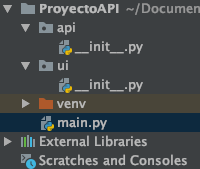
\includegraphics[width=0.45\textwidth]{Images/arq_proyecto.png}
    \caption{Estructura Base de la Arquitectura Modular}
    \label{fig:arquitectura}
\end{figure}

El árbol de directorios definitivo del proyecto es el siguiente:
\begin{lstlisting}[language=bash]
proyecto_suelos/
|-- api/
|   |-- __init__.py
|   `-- data_service.py       # Logica de negocio y medianas
|-- ui/
|   |-- __init__.py
|   `-- cli_view.py           # Interfaz de consola
|-- data/
|   `-- resultado_laboratorio_suelo.xlsx # Dataset oficial
|-- tests/
|   |-- __init__.py
|   `-- test_api.py           # Suite de pruebas unitarias
|-- main.py                   # Punto de entrada
|-- requirements.txt          # Dependencias
`-- README.md                 # Documentacion tecnica
\end{lstlisting}

\newpage
\section{Evidencias de Funcionamiento y Pruebas}

\subsection{Pruebas Unitarias Automatizadas}
Se ejecutó la suite de pruebas unitarias implementada en \texttt{tests/test\_api.py}, validando la normalización de texto, la limpieza de datos corruptos, el cálculo sintético de la mediana y la consulta contra el dataset oficial:

\begin{lstlisting}[language=bash]
$ python -m unittest tests/test_api.py
....
----------------------------------------------------------------------
Ran 4 tests in 0.174s

OK
\end{lstlisting}

\subsection{Consultas Realizadas en el Departamento de Risaralda}

\subsubsection{Caso 1: Cultivo de Aguacate en el Municipio de Pereira}
\begin{lstlisting}[language=bash]
$ python main.py -d "Risaralda" -m "Pereira" -c "Aguacate" -l 5

+----------------+-------------+-----------+--------------+--------------+-------------------+----------------+
| Departamento   | Municipio   | Cultivo   | Topografia   |   Mediana pH |         Mediana P |      Mediana K |
|                |             |           |              |              |   (Bray II mg/kg) |   (cmol(+)/kg) |
+================+=============+===========+==============+==============+===================+================+
| RISARALDA      | PEREIRA     | Aguacate  | Ondulado     |         4.95 |             68.66 |          0.107 |
| RISARALDA      | PEREIRA     | Aguacate  | Ondulado     |         4.95 |             68.66 |          0.107 |
| RISARALDA      | PEREIRA     | Aguacate  | Ondulado     |         4.95 |             68.66 |          0.107 |
| RISARALDA      | PEREIRA     | Aguacate  | Ondulado     |         4.95 |             68.66 |          0.107 |
| RISARALDA      | PEREIRA     | Aguacate  | Ondulado     |         4.95 |             68.66 |          0.107 |
+----------------+-------------+-----------+--------------+--------------+-------------------+----------------+
\end{lstlisting}

\subsubsection{Caso 2: Cultivo de Caña en el Municipio de Balboa}
\begin{lstlisting}[language=bash]
$ python main.py -d "Risaralda" -m "Balboa" -c "Cana" -l 5

+----------------+-------------+----------------------+--------------+--------------+-------------------+----------------+
| Departamento   | Municipio   | Cultivo              | Topografia   |   Mediana pH |         Mediana P |      Mediana K |
|                |             |                      |              |              |   (Bray II mg/kg) |   (cmol(+)/kg) |
+================+=============+======================+==============+==============+===================+================+
| RISARALDA      | BALBOA      | Cana panelera/azucar | Plano        |         6.55 |             49.28 |          0.267 |
| RISARALDA      | BALBOA      | Cana panelera/azucar | Plano        |         6.55 |             49.28 |          0.267 |
| RISARALDA      | BALBOA      | Cana panelera/azucar | Plano        |         6.55 |             49.28 |          0.267 |
| RISARALDA      | BALBOA      | Cana panelera/azucar | Plano        |         6.55 |             49.28 |          0.267 |
| RISARALDA      | BALBOA      | Cana panelera/azucar | Plano        |         6.55 |             49.28 |          0.267 |
+----------------+-------------+----------------------+--------------+--------------+-------------------+----------------+
\end{lstlisting}

\subsubsection{Caso 3: Cultivo de Café en Santa Rosa de Cabal}
\begin{lstlisting}[language=bash]
$ python main.py -d "Risaralda" -m "Santa Rosa" -c "Cafe" -l 3

+----------------+-------------+-----------+--------------+--------------+-------------------+----------------+
| Departamento   | Municipio   | Cultivo   | Topografia   |   Mediana pH |         Mediana P |      Mediana K |
|                |             |           |              |              |   (Bray II mg/kg) |   (cmol(+)/kg) |
+================+=============+===========+==============+==============+===================+================+
| RISARALDA      | SANTA ROSA  | Cafe      | Ondulado     |         5.42 |              3.87 |           0.08 |
+----------------+-------------+-----------+--------------+--------------+-------------------+----------------+
\end{lstlisting}

\end{document}
